\documentclass{tstextbook}

% Template from http://www.typesetters.se/latex-textbook-template/ 
\usepackage{multicol}

\begin{document}

\begin{titlepage}
\BgThispage
\newgeometry{left=1cm,right=6cm,bottom=2cm}
\vspace*{0.4\textheight}
\noindent
\textcolor{white}{\Huge\textbf{\textsf{Math 1}}}
\vspace*{2cm}\par
\noindent
\begin{minipage}{0.35\linewidth}
    \begin{flushright}
    Nantucket High School \\
    2022 -- 2023
    \end{flushright}
\end{minipage} \hspace{15pt}
%
\begin{minipage}{0.02\linewidth}
    \rule{1pt}{175pt}
\end{minipage} \hspace{-10pt}
%
\begin{minipage}{0.63\linewidth}
\vspace{5pt}
%    \begin{abstract} 
%  
\hspace{35mm}
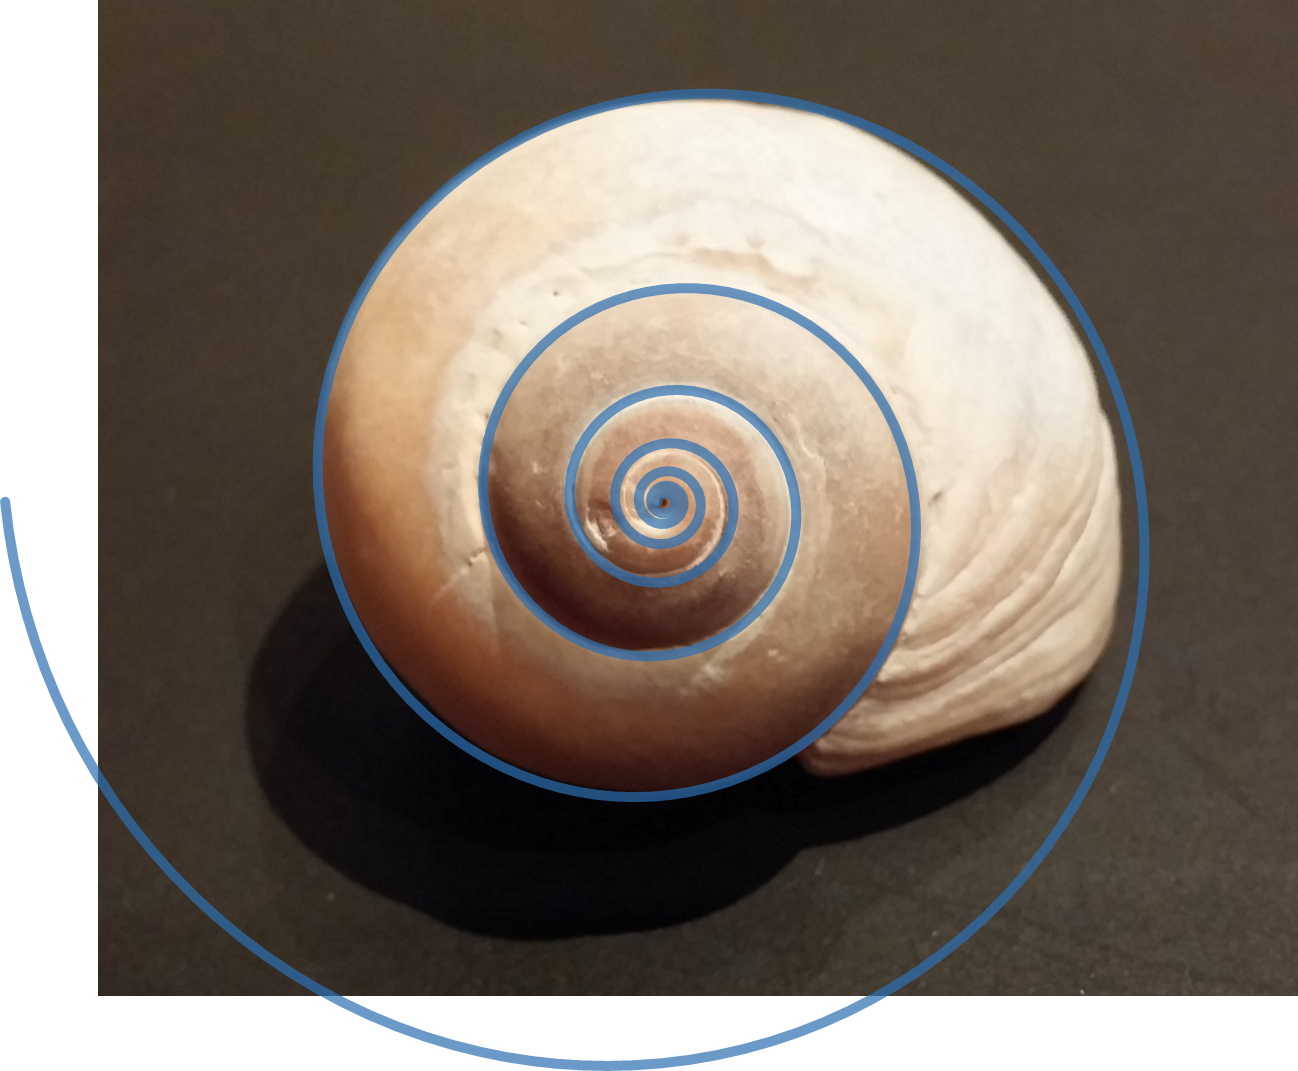
\includegraphics[width=1.0\textwidth]{img/shell.png}
%    \end{abstract}
\end{minipage}
\end{titlepage}

\newpage

%%%%%%%%%%%%%%%%%%%%%%%%%%%%%%%%%%%%%%%

\pagenumbering{gobble}

\setcounter{section}{-1}

\null\vfill
\noindent
%Copyright 2022 \textsuperscript \textcopyright \ 
Nantucket High School 
%Jedediyah Williams
%williamsj@npsk.org
\\ \\
\textbf{Copying this document is encouraged} 
\\ \\ 
Licensed under the Creative Commons Attribution-NonCommercial 4.0 International license; 
\\ 
    You are free to: 
    
    Share — copy and redistribute the material in any medium or format; Adapt — remix, transform, and build upon the material.  
    
    Attribution — You must give appropriate credit, provide a link to the license, and indicate if changes were made. You may do so in any reasonable manner, but not in any way that suggests the licensor endorses you or your use. 
    
    NonCommercial — You may not use the material for commercial purposes. 
    \\ \\
    https://creativecommons.org/licenses/by-nc/4.0/
    
    
\newpage

\newpage
\section*{Acknowledgements}

Thanks to http://www.typesetters.se/latex-textbook-template/ for the \LaTeX \ template.
\\ \\
Thanks to https://tex.stackexchange.com/questions/85904/showcase-of-beautiful-title-page-done-in-tex for the \LaTeX \ title page template.

\newpage
\section*{Introduction}

How to be successful at learning:
\\ \vspace{5mm}

\noindent
\textbf{Attend} \\ 
Class time is valuable.  
Sometimes you will miss class, so always check-in to see what you’ve missed.  Keep your work organized and don’t miss out on opportunities for learning.  
Minimize distractions and your learning will be substantially more efficient and effective.
\\ \vspace{5mm}

\noindent
\textbf{Think} \\
Our goal is for you to learn!  Learning is a change in your long-term memory, and “memory is the residue of thought" {\small (\url{https://www.aft.org/sites/default/files/periodicals/willingham_0.pdf}) }.
We will pose ideas and demonstrate techniques, but the learning happens in your head.  
That learning is your responsibility and the way to learn is to process information critically through thought.
Consistently ask yourself questions like "how does this work?" and "when does this not work?".
\\ \vspace{5mm}

\noindent
\textbf{Practice} \\  
We practice to improve.  
Think about playing an instrument, drawing, or playing a sport.  
A common mistake in mathematics is to think that something “makes sense” so you stop practicing it.  
You will see things that seem easy and you will see things that seem challenging.  
In both cases, practice is essential.  
We may be showing you something with which you are already familiar because there is a deeper understanding to be found!  
If something seems challenging, we are practicing it so that we can move toward mastering it.  
\\ \vspace{5mm}

\noindent
\textbf{Academic Integrety} \\ 
Academic integrity is paramount. 
Academic dishonesty includes any participation in cheating, helping someone else cheat, or in any way misrepresenting your knowledge by submitting or manipulating your work or the work of others. 

\newpage 
\tableofcontents
\newpage
\pagenumbering{arabic}

%
%---------------------------------------------------------------------------
\chapter{First chapter}

\begin{summary}
  This first chapter illustrates how to use various elements of this
  text book template, such as definitions, theorems and exercises. You
  may want to start each chapter with a meta summary like this one, to
  explain to the reader what the chapter is all about, why it is
  important and how it fits into the bigger picture of the
  book. Another useful tip is to put the contents of each chapter into
  a separate \LaTeX{} file and then use the command
  \texttt{\textbackslash{}input\{\}} to include the chapter in the
  main document.
\end{summary}

\section{First section}

Let's start out with the following theorem.

\begin{theorem}[Logic algebra]
  \label{th:logicalgebra}
  \index{logic algebra}
  Let $P$, $Q$ and $R$ be logical propositions (true or false).
  Then the following propositions are true:
  \small
  \begin{align*}
    P \land Q &\Leftrightarrow Q \land P &
    P \lor  Q &\Leftrightarrow Q \lor P  &&
    \text{(commutative laws)} \\
    (P \land Q) \land R &\Leftrightarrow P \land (Q \land R) &
    (P \lor Q)  \lor  R &\Leftrightarrow P \lor  (Q \lor  R) &&
    \text{(associative laws)} \\
    P \land (Q \lor  R) &\Leftrightarrow (P \land Q) \lor  (P \land R) &
    P \lor  (Q \land R) &\Leftrightarrow (P \lor  Q) \land (P \lor  R) &&
    \text{(distributive laws)} \\
    \lnot (P \land Q) &\Leftrightarrow \lnot P \lor  \lnot Q &
    \lnot (P \lor  Q) &\Leftrightarrow \lnot P \land \lnot Q &&
    \text{(De Morgan's laws)}
  \end{align*}
\end{theorem}
\begin{proof}
  \newcommand{\T}{\mathsf{T}}
  \newcommand{\TT}{\mathbf{T}}
  \renewcommand{\F}{\mathsf{F}}
  We prove the first of De Morgan's laws and leave the proofs of
  the remaining propositions as exercises. To prove the statement,
  we create a truth table and fill in all possible values (true or
  false) for the propositions $P$ and $Q$. Each of these propositions
  can be either true or false and we thus obtain the following truth
  table with four cases:
  \begin{center}
    \begin{tabular}{cccccccccc}
      $\lnot$ & ($P$ & $\land$ & $Q$) & $\Leftrightarrow$ & $\lnot$ & $P$ & $\lor$ & $\lnot$ & $Q$ \\
      \midrule
      & $\T$ && $\T$ &&& $\T$ &&& $\T$ \\
      & $\T$ && $\F$ &&& $\T$ &&& $\F$ \\
      & $\F$ && $\T$ &&& $\F$ &&& $\T$ \\
      & $\F$ && $\F$ &&& $\F$ &&& $\F$
    \end{tabular}
  \end{center}
  By definition of the logical operators, we compete the table to obtain
  \begin{center}
    \begin{tabular}{cccccccccc}
      $\lnot$ & ($P$ & $\land$ & $Q$) & $\Leftrightarrow$ & $\lnot$ & $P$ & $\lor$ & $\lnot$ & $Q$ \\
      \midrule
      $\F$ & $\T$ & $\T$ & $\T$ & $\TT$ & $\F$ & $\T$ & $\F$ & $\F$& $\T$ \\
      $\T$ & $\T$ & $\F$ & $\F$ & $\TT$ & $\F$ & $\T$ & $\T$ & $\T$& $\F$ \\
      $\T$ & $\F$ & $\F$ & $\T$ & $\TT$ & $\T$ & $\F$ & $\T$ & $\F$& $\T$ \\
      $\T$ & $\F$ & $\F$ & $\F$ & $\TT$ & $\T$ & $\F$ & $\T$ & $\T$& $\F$
    \end{tabular}
  \end{center}
  It follows that the statement we want to prove (the equivalence $\Leftrightarrow$)
  is always true (a \emph{tautology}), which proves the statement.
\end{proof}

\section{Second section}

We begin our next section with the following central definition.

\begin{definition}[Rational Cauchy sequence]
  \label{th:rationalcauchysequence}
  \index{rational Cauchy sequence}
  A rational Cauchy sequence is a rational sequence
  $(x_n)_{n=0}^{\infty}$ such that
  \begin{equation}
    \forall \epsilon \in \mathbb{Q}_+ \;
    \exists N \in \mathbb{N} : m, n \geq N \Rightarrow |x_m - x_n| < \epsilon.
  \end{equation}
  In other words, for each (small) rational number $\epsilon > 0$
  there is a (big) number $N$ such that the distance $|x_m - x_n|$
  between $x_m$ and $x_n$ is less than $\epsilon$ if both $m$ and $n$
  are larger than or equal to $N$.
\end{definition}

\begin{remark}
  A remark may be in order here. This definition is concerned with
  \emph{rational} Cauchy sequences. We will later encounter a similar
  definition of \emph{real} Cauchy sequences.
\end{remark}

\begin{example}[Solving the equation $x^2 = 2$]
  Consider the equation $x^2 = 2$. It is easy to prove that this
  equation does not have any rational solutions. However, consider
  the following iteration formula:
  \begin{equation}
    x_n = \frac{x_{n-1} + 2 / x_{n - 1}}{2},
  \end{equation}
  where $n = 1,2,3,\ldots$ and $x_0 = 1$. The resulting sequence of
  rational numbers quickly approaches a number in the vicinity of
  $x = 1.4142135623731$:
  \begin{displaymath}
    \begin{array}{rclcl}
      x_0 &=& 1 \\
      x_{1} &=& (x_{0} + 2 / x_{0}) / 2 &=& 1.5 \\
      x_{2} &=& (x_{1} + 2 / x_{1}) / 2 &\approx& 1.4166666666667 \\
      x_{3} &=& (x_{2} + 2 / x_{2}) / 2 &\approx& 1.4142156862745 \\
      x_{4} &=& (x_{3} + 2 / x_{3}) / 2 &\approx& 1.4142135623747 \\
      x_{5} &=& (x_{4} + 2 / x_{4}) / 2 &\approx& 1.4142135623731 \\
      x_{6} &=& (x_{5} + 2 / x_{5}) / 2 &\approx& 1.4142135623731 \\
      x_{7} &=& (x_{6} + 2 / x_{6}) / 2 &\approx& 1.4142135623731 \\
      x_{8} &=& (x_{7} + 2 / x_{7}) / 2 &\approx& 1.4142135623731 \\
      x_{9} &=& (x_{8} + 2 / x_{8}) / 2 &\approx& 1.4142135623731 \\
      x_{10} &=& (x_{9} + 2 / x_{9}) / 2 &\approx& 1.4142135623731
    \end{array}
  \end{displaymath}
  We will later see that this iteration, or any other equivalent
  iteration, defines the real number $\sqrt{2}$.
\end{example}

\section{Third section}

Now let's move on to the definition of the real number system. This
may be defined in a multitude of ways, one of which is to think about
a real number as a rational Cauchy sequence, or rather the equivalence
class of Cauchy sequences ``converging to'' that number.

\begin{definition}[The real numbers $\mathbb{R}$]
  \label{def:realnumbers}
  \index{real numbers}
  The real numbers $\mathbb{R}$ is the set of all equivalence classes
  of rational Cauchy sequences.
\end{definition}

Now that this is settled, lets prove the completeness of the real
number system.

\begin{theorem}[The completeness of the real numbers]
  \label{th:realnumberscomplete}
  \index{completeness of the real numbers}
  Let $(x_n)_{n=0}^{\infty}$ be a sequence of real numbers.
  Then $(x_n)_{n=0}^{\infty}$ is convergent if and only if
  it is also a real Cauchy sequence.
  \end{theorem}
\begin{proof}
  Write $x_m = [(x_{mn})_{n=0}^{\infty}]$ where
  $x_{mn}$ is the $n$th number in a rational Cauchy sequence
  representing the real number $x_m$. And so on\ldots.
\end{proof}

For further reading, there are several excellent works that one could
cite, such as \cite{Tao2006,Turing1936}.

\section*{Exercises}

\begin{exercise}
  Let $A = \{1, 2, 3\}$ and $B = \{2, 3, 4\}$.
  Determine the following sets. \\
  (a) $A \cup B$ \quad
  (b) $A \cap B$ \quad
  (c) $A \setminus B$ \quad
  (d) $A \times B$
\end{exercise}

\begin{exercise}
  Let $A = \{1, 3, 5, 7, 9\}$ and $B = \{2, 4, 6, 8, 10\}$.
  Determine the following sets. \\
  (a) $A \cup B$ \quad
  (b) $A \cap B$ \quad
  (c) $A \setminus B$ \quad
  (d) $A \times B$
\end{exercise}

\begin{exercise}
  Let $A = \{1, 2, 3\}$, $B = \{2, 3, 4\}$ and $C = \{3, 4, 5\}$.
  Determine the following sets. \\
  (a) $A \cup B \cup C$ \quad
  (b) $A \cap B \cap C$ \quad
  (c) $(B \setminus A) \cap C$ \quad
  (d) $(A \times B) \times C$
\end{exercise}

\section*{Problem}

\begin{problem}
  Interpret the following set definition (Russell's paradox) and discuss
  whether $X \in X$ or $X \notin X$:
  \begin{equation}
    X = \{x \mid x \notin x\}.
  \end{equation}
\end{problem}

\section*{Computer exercises}

\begin{programming}
  Write a program that generates the sequence $(x_n)_{n=0}^{100}$
  for $x_n = n$.
\end{programming}

\begin{programming}
  Write a program that generates the odd numbers between $1$ and $100$.
\end{programming}

\begin{programming}
  Write a program that computes the sum $\sum_{n=0}^{100} x_n$
  for $x_n = n$.
\end{programming}

%---------------------------------------------------------------------------
\chapter{Second chapter}

\begin{summary}
  \blindtext
\end{summary}

\section{First section}
\Blindtext

\section{Second section}
\Blindtext

\section{Third section}
\Blindtext

%---------------------------------------------------------------------------
\chapter{Third chapter}

\begin{summary}
  \blindtext
\end{summary}

\section{First section}
\Blindtext

\section{Second section}
\Blindtext

\section{Third section}
\Blindtext

  % Uncomment to see style examples 

%%%%%%%%%%%%%%%%%%%%%%%%%%%%%%%%%%%%


%%%%%%%%%%%%%%%%%%%%%%%%%%%%%%%%%%%%%%
% Chapter title 
\chapter{Number and Expression}

% Chapter summary 
\begin{summary}
In this chapter, we will:
\begin{itemize}
    \item Write numbers using decimals, negatives, and fractions
    \item Add, subtract, multiply, and divide
    \item Expand and rewrite terms using exponents
    \item Find and approximate square and cube roots
    \item Simplify expressions in order of operations 
    \item Use variables to represent unknown quantities
    \item Evaluate variable expressions
    
\end{itemize}
\end{summary}

% Chapter contents 


%%%%%%%%%%%%%%%%%%%%%%%%%
\newpage 
\section{Numbers}

\subsection{Negatives}
\begin{definition}[Negative]
The \emph{negative} of a number is its \emph{opposite}, and has the same distance from zero on the number line.  The opposite of \(58\) is \(-58\).  The opposite of \(-27.3\) is \(27.3\).  
\end{definition}

While not the same as subtraction, negative numbers can be viewed as positive numbers being subtracted from \(0\), an idea that will be useful when we start to perform arithmetic with negative numbers.  

\subsubsection{Adding and Subtracting} 
Adding a positive number is equivalent to moving ``right'' or ``up'' the number line.  
Draw a number line diagram for each of the operations below. 
\[10 + 2 = 12  \]
%\[80+19 = 99   \]
\[ 108 + 15 = 123  \]
%\[  -8 + 3 = -5 \]
\[  -15 + 5 = -10   \]
%\[  -8 + 20 = 12 \]
Note that even when starting with a negative, adding a positive number still moves ``up''. 

Subtracting a positive number is equivalent to moving ``left'' or ``down'' the number line. 
Draw a number line diagram for each of the operations below. 
\[ 38 - 11 = 27 \]
\[  5-8 = -3  \]
\[  -7 - 4 = -11   \]
Adding a negative can be translated to subtraction.  For example, 
\[10 + (-2) = 10 -2 = 8 \]
\[  17 + (-8) = 9 \]
Subtracting a negative can be translated to addition.  For example, 
\[  22 - (-4) = 26 \]
\[ -7 - (-2) = -5 \]

\subsubsection{Multiplying and Dividing} 
There are four cases to consider: 
\[ (+)(+) \to (+)  \]
\[ (+)(-) \to (-)  \]
\[ (-)(+) \to (-)  \]
\[ (-)(-) \to (+)  \]
Justify each of these cases for multiplication.  The same justifications will hold for division.  

%%%%%%%%%%%%%%%%%%%%%%%%%
\newpage 

\begin{exercise}
	Draw a number line diagram for each of the following operations:   \\ \\
(a)	\[  12 + 7  \]    
(b)	\[  8 + (-10) \]  
(c)	\[  -3 - 4  \]
(d)	\[  -2 - (-7)    \]

\end{exercise}



%%%%%%%%%%%%%%%%%%%%%%%%%
\newpage 
\subsection{Factors}
\begin{definition}[Factor]
The \emph{factors} of any number \(n\) are the numbers that can be multiplied to get \(n\).  

For example, the factors of \(8\) are \(1, 2, 4, \text{ and } 8\). When we say ``factors'', we are usually referring to positive whole-number factors. 
\end{definition}

\begin{figure}[h!]
    \centering
    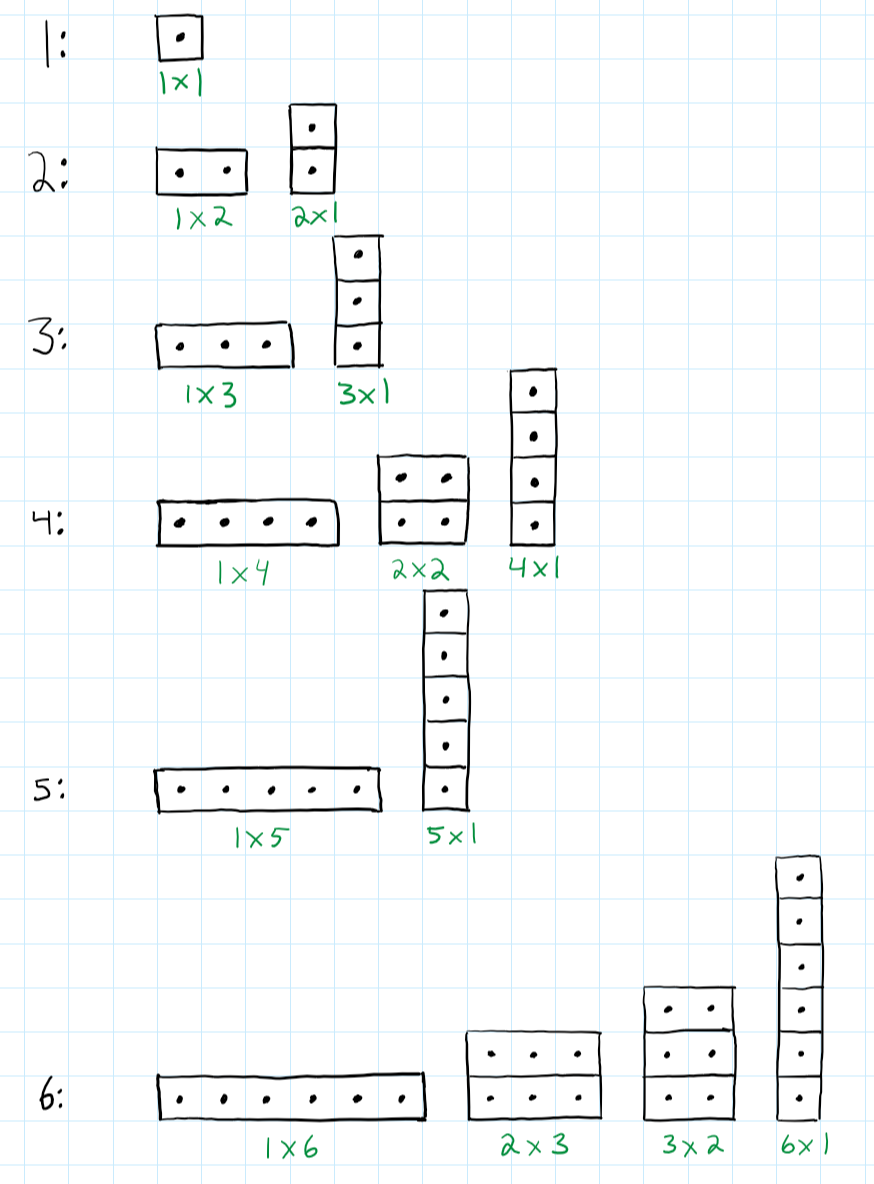
\includegraphics[width=0.7\textwidth]{img/number_factors.png}  
    % Source: Jed
    \caption{Factoring diagrams for \(1\) through \(6\).}
    \label{fig:number-factors}
\end{figure}
\begin{exercise}
	Figure~\ref{fig:number-factors} depicts factoring diagrams of numbers \(1\) through \(6\).  
	Make the factoring diagrams for numbers up through at least \(18\).  
	\\ \hspace*{15mm}(a) What do you notice?
	\\ \hspace*{15mm}(b) What do you wonder? 
\end{exercise}



%%%%%%%%%%%%%%%%%%%%%%%%%
\newpage 
Observing our factoring diagrams in Figure~\ref{fig:number-factors}, some numbers can only be diagramed in two ways.  For example, \(7\) can only be written as \(1 \times 7\) and \(7 \times 1\).  In other words, the only factors of \(7\) are \(1\) and \(7\) itself.  We call such numbers \emph{prime numbers}.  Numbers that have additional number factors are called \emph{composite numbers}.   
\vspace{3mm}
\begin{exercise}
	Primes
	\\ \hspace*{15mm} (a) Write down as many primes as you can in about a minute!
	\\ \hspace*{15mm} (b) Write down three questions about prime numbers. 
	\label{ex:primelist}
\end{exercise}
\vspace{5mm}
We (humanity) know a lot about primes. 
As much as we know, there is much more that we do not know!  There are many \emph{open problems} regarding primes.  The Riemann hypothesis, one of the most famous unsolved problems in mathematics, is related to the distribution of prime numbers.  When moving along the number line, there is no known efficient method for predicting how many numbers will pass before the next prime.  If you were to find such a pattern, you would be instantly famous!  
\vspace{3mm}
\begin{exercise} \textbf{Factors: Looking for Patterns in Primes}
\\ \\
(a) Create a list of factors for the numbers up to at least \(20\), and keep count of the number of factors.  
\[ 
	\begin{array}{c | l | c}
		n & \text{Factors} & \text{Count} \\ \hline 		 
		1 & 1  & 1\\ 
		2 & 1, 2 & 2\\ 
		3 & 1, 3 & 2\\ 
		4 & 1, 2, 4 & 3\\
		5 & 1, 5 & 2 \\
		6 & 1, 2, 3, 6 & 4 \\ 
		\vdots & \vdots & \vdots  \\
	\end{array}
\]
(b) Create a ``grid'' chart of factors.  Label the horizontal and vertical axes \(1\) through \(20\).  For each number on the horizontal axis, fill in the square corresponding to each of its factors in the vertical direction.  
\\ 
(c) What patterns do you observe, and do you expect they continue?  What future paterns do you expect might arrise?
\label{ex:primepatterns}
\end{exercise}
\subsubsection{Resources}
\begin{itemize}
	\item {\footnotesize ``Michael Says Prime Numbers for 3 Hours'', \url{https://www.youtube.com/watch?v=NHEaYbDWyQE}}
	\item {\footnotesize ``Sieve of Eratosthenes'', \url{https://en.wikipedia.org/wiki/Sieve_of_Eratosthenes}}
	\item {\footnotesize ``The Prime Number Spiral (Coding Challenge 167)'', \url{https://www.youtube.com/watch?v=a35KWEjRvc0}}
	\item {\footnotesize ``How they found the World's Biggest Prime Number'', \url{https://www.youtube.com/watch?v=lEvXcTYqtKU}}
	\item {\footnotesize ``Encryption and HUGE numbers - Numberphile'', \url{https://www.youtube.com/watch?v=M7kEpw1tn50}}
	\item {\footnotesize ``Riemann Hypothesis - Numberphile'', \url{https://www.youtube.com/watch?v=d6c6uIyieoo}}
\end{itemize}

%%%%%%%%%%%%%%%%%%%%%%%%%
\newpage 
\subsection{GCF and LCM}

\begin{definition} [Greatest Common Factor]
The \emph{greatest common factor} (GCF) of two numbers is the largest factor they have in common.  

For example, The GCF of \(8\) and \(12\) is \(4\). The GCF of \(9\) and \(27\) is \(9\).  
\end{definition}
One strategy for finding the GCF of two numbers is to list each of their factors, eliminate all but those in common, and then identify the largest.  
\begin{example}\textbf{Find the GCF of 16 and 24}
\\ 
The factors of \(16\) are 
\[1,2, 4, 8, 16\]
The factors of \(24\) are 
\[ 1, 2, 3, 4, 6, 8, 12, 24 \]
The greatest common factor of \(16\) and \(24\) is \(8\). 
\end{example}
\begin{exercise}
Create a \(10 \times 10\) grid.  For each square in the grid, write the GCF of the corresponding numbers at that square.  
	\\ \hspace*{15mm}(a) What do you notice?
	\\ \hspace*{15mm}(b) What do you wonder? 
\\
You can turn your grid into a 3D visualization of GCF by stacking objects (coins, dice, etc.) on each squares according to the GCF value on that square. 
\label{ex:gcdgrid}
\end{exercise}

\begin{definition} [Least Common Multiple]
The \emph{least common multiple} (LCM) of two numbers is the smallest multiple they have in common.  

For example, the LCM of \(6\) and \(4\) is \(12\).  The LCM of \(8\) and \(24\) is \(24\).   
\end{definition}


%%%%%%%%%%%%%%%%%%%%%%%%%
\newpage 
\subsection{Fractions}
There are many ways to think about fractions: we can talk about fractions as part of a whole, or as a ratio, or rate, or as division.  
\begin{figure}[h!]
    \centering
    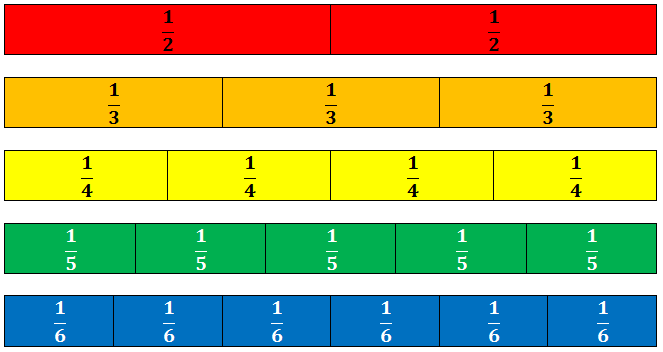
\includegraphics[width=0.7\textwidth]{img/FractionStrips.png}  
    % Source: https://commons.wikimedia.org/wiki/File:FractionStrips.PNG 
    \caption{Fraction Strips. The width is a whole.}
    \label{fig:fraction-strips}
\end{figure}
\\
A lot of concepts we'll work with revolve around \emph{equivalent fractions}, fractions that are equivalent!
\begin{figure}[h!]
    \centering
    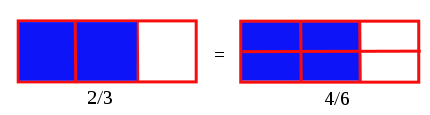
\includegraphics[width=0.5\textwidth]{img/fraction2-3.png}
    % Source: https://commons.wikimedia.org/wiki/File:Fraction2_3.svg
    \caption{Equivalent Fractions.  The fraction \(\frac{2}{3}\) is equivalent to the fraction \(\frac{4}{6}\).}
    \label{fig:equivalent-fractions}
\end{figure}
\\ 
% REDUCE 
\textbf{Reducing Fractions}
\\ \\ 
\emph{Reducing} is one of the most common tasks we'll see with fractions.  Reducing a fraction means to write a fraction in its lowest terms.  




%%%%%%%%%%%%%%%%%%%%%%%%%%%%%%%
\newpage 
\textbf{Adding and Subtracting Fractions}
\\ \\
Adding fractions involves combining numerators.   The example below could be read as ``five eigths plus two eigths equals seven eigths''.  
\begin{example}
	Find the following sum:
	\[\frac{5}{8}+\frac{2}{8}\]
\textbf{Solution:}
	\[\frac{5}{8}+\frac{2}{8} = \frac{5+2}{8} =  \frac{7}{8}\]
\end{example}
\vspace{3mm}
Subtraction is similar. 
\begin{example}
	Find the following difference:
	\[\frac{5}{8}-\frac{2}{8}\]
\textbf{Solution:}
	\[\frac{5}{8}-\frac{2}{8} = \frac{5-2}{8} = \frac{3}{8}\]
\end{example}
\vspace{3mm}
Adding and subtracting fractions requires a common denominator.  For example, we cannot cannot directly add or subtract thirds with fifths.  However, we can convert fractions to equivalent fractions with common denominators.  
\begin{example}
	Find the following sum: 
	\[\frac{7}{3} + \frac{2}{5}\]
\textbf{Solution:}
	\[\frac{7}{3} + \frac{2}{5} = \frac{35}{15} + \frac{14}{15} = \frac{49}{15} \]
\end{example}
To get a common denominator, you want to determine the smallest common multiple of your two denominators.  That is, the smallest number that is a multiple of both denominators.  In the example above, \(15\) is a multiple of both \(3\) and \(5\).  
\begin{remark}
 	When converting a fraction to an equivalent fraction, we can think of this manipulation as multiplying by \(1\).  For example, we coverted \(\frac{7}{3}\) to \(\frac{35}{15}\) by multiplying \(\frac{7}{3}\) by \(\frac{5}{5}\).  Importantly, \(\frac{5}{5} = 1\)  and multiplying by \(1\) does not change the \emph{value} of the original number. 
\end{remark}



%%%%%%%%%%%%%%%%%%%%%%%%%%%%%%%
\newpage 


\begin{exercise}
	Find the missing terms of these sums. 

	(a)	\[\frac{5}{12} + \frac{1}{12} = \frac{ }{12} \]
	(b)	\[\frac{ }{9} + \frac{2}{9} = \frac{13}{9} \]
	(c)	\[\frac{4}{3} + \frac{11}{3} = \text{---} \]
%	{\footnotesize \url{https://www.khanacademy.org/math/cc-fourth-grade-math/imp-fractions-2/imp-adding-and-subtracting-fractions-with-like-denominators/e/adding_fractions_with_common_denominators}}
\\ 
	{\footnotesize \url{https://www.ixl.com/math/grade-4/add-fractions-with-like-denominators-using-area-models}}
\end{exercise} 
\begin{exercise}
	Find the missing terms in these differences.  
	
	(a)	\[\frac{5}{12} - \frac{1}{12} = \frac{}{12} \]
	(b)	\[\frac{7}{9} - \frac{2}{9} = \text{---}  \]
	(c)	\[\frac{11}{3} - \frac{-4}{3} = \text{---} \]
\\ 
%	{\footnotesize \url{https://www.khanacademy.org/math/cc-fourth-grade-math/imp-fractions-2/imp-adding-and-subtracting-fractions-with-like-denominators/e/subtracting_fractions_with_common_denominators}}
	{\footnotesize \url{https://www.ixl.com/math/grade-4/subtract-fractions-with-unlike-denominators}}
\end{exercise} 
\begin{exercise}
	Find the missing terms in these sums and differences.  
	
	(a)	\[\frac{5}{6} + \frac{1}{2} = \frac{5}{6} + \frac{}{6} = \frac{}{6} \]
	(b)	\[\frac{7}{9} - \frac{2}{9} = \text{---}  \]
	(c)	\[\frac{11}{3} - \frac{4}{3} = \text{---} \]
\\ 	
	{\footnotesize \url{https://www.ixl.com/math/grade-6/add-and-subtract-fractions-with-unlike-denominators}}
\end{exercise} 
Additional Practice: 
\begin{itemize}
	\item {\footnotesize \url{https://www.ixl.com/math/grade-3/add-and-subtract-fractions-with-like-denominators}}
	\item {\footnotesize \url{https://www.ixl.com/math/grade-4/add-3-or-more-fractions-with-unlike-denominators}}
\end{itemize}





%%%%%%%%%%%%%%%%%%%%%%%%%%%%%%%
\newpage 
\textbf{Multiplying and Dividing Fractions}
\\ \\ 
Unlike addition and subtraction, multiplication and division of fractions do not require common denominators.  





%%%%%%%%%%%%%%%%%%%%%%%%%
\newpage 
\section{Operations}

Adding, subtracting, multiplying, and dividing are all \emph{operations} on numbers.  In this section, we'll see some additional operations including exponentiation, square roots, and cube roots.  

%\subsection{Multiplying and Dividing}
\subsection{Exponents and Roots} 
\emph{Exponents} corresponds to repeated multiplication.  
A negative exponent corresponds to repeated division.  
Consider the following examples:
\[ 3^{4} = 1 \cdot 3 \cdot 3 \cdot 3 \cdot 3   \]
\[ 3^{3} = 1 \cdot 3 \cdot 3 \cdot 3    \]
\[ 3^{2} = 1 \cdot 3 \cdot 3   \]
\[ 3^{1} = 1 \cdot 3    \]
\[ 3^{0} = 1    \]
\[ 3^{-1} = 1 / 3  \]
\[ 3^{-2} = 1 / 3 / 3 \]
Here are some additonal examples!
\[ 4^{3} = 64 \]
\[ 3^{3} = 27  \]
\[ 5^{-2} = \frac{1}{25}  \]
\[  15^{-3} = \frac{1}{3375} \]
\begin{exercise}
	Evaluate the following exponents.
	\\ \hspace*{15mm} (a) \( 2^{8} \)
	\label{ex:basicexponents}
\end{exercise}


%%%%%%%%%%%%%%%%%%%%%%%%%
\newpage 
\subsection{Order of Operations}


%%%%%%%%%%%%%%%%%%%%%%%%%
\newpage 
\subsection{Application: Pythagorean Theorem} 

\begin{theorem} \textbf{Pythagorean Theorem} \\ 
If and only if a triangle is a right-triangle, with legs \(a\) and \(b\) and hypotenuse \(c\),
\[a^2 + b^2 = c^2\]
\end{theorem}


%%%%%%%%%%%%%%%%%%%%%%%%%
\newpage 
\section{Expressions}

\subsection{Variables}
\subsection{Evaluating Expressions}
\subsection{Equivalent Expressions}
\subsubsection{Combining Like-Terms}

%%%%%%%%%%%%%%%%%%%%%%%%%
\newpage 
\section{Exercises} 

Online Practice from this Chapter ... 

Additional problems. 


















%%%%%%%%%%%%%%%%%%%%%%%%%%%%%%%%%%%%%%
% Chapter title 
\chapter{Equivalence}

% Chapter summary 
\begin{summary}
In this chapter, we will:
\begin{itemize}
    \item Utilize equality to manipulate multiple expressions
    \item Solve equations for variable quantities 
\end{itemize}

Equality is at the heart of Algebra. 
\end{summary}

% Chapter contents 


%%%%%%%%%%%%%%%%%%%%%%%%%
\newpage 
\section{Balancing Equations}



%%%%%%%%%%%%%%%%%%%%%%%%%
\newpage 
\section{Solving Equations}

\subsection{One-Step}
\subsection{Two-Step}
\subsection{Multi-Step}


%%%%%%%%%%%%%%%%%%%%%%%%%
\newpage 
\section{Exercises} 

%%%%%%%%%%%%%%%%%%%%%%%%%%%%%%%%%%%%%%
% Chapter title 
\chapter{Linear Equations and Inequalities}

% Chapter summary 
\begin{summary}
In this chapter, we will: 
\begin{itemize}
    \item 
\end{itemize}
\end{summary}

% Chapter contents 
\newpage 

%%%%%%%%%%%%%%%%%%%%%%%%%
\section{Linear Equations}

\subsection{Equations, Tables, and Graphs}
\subsection{Properties of Lines}


%%%%%%%%%%%%%%%%%%%%%%%%%
\newpage 
\section{Application: Modeling}
    \subsection{Bounce Height}

%%%%%%%%%%%%%%%%%%%%%%%%%
\newpage 
\section{Linear Inequalities}


%%%%%%%%%%%%%%%%%%%%%%%%%
\newpage 
\section{Exercises} 

%%%%%%%%%%%%%%%%%%%%%%%%%%%%%%%%%%%%%%
% Chapter title 
\chapter{Systems}

% Chapter summary 
\begin{summary}
In this chapter, we will 
\begin{itemize}
    \item 
\end{itemize}
\end{summary}

% Chapter contents 

\newpage 
%%%%%%%%%%%%%%%%%%%%%%%%%
\section{Systems of Equations}

What is a solution to a system of equations?

\subsection{Graphical Solutions}
Finding solutions graphically

\subsection{Analytical Solutions: Substituion and Elimination}
Finding solutions analytically 


\newpage 
%%%%%%%%%%%%%%%%%%%%%%%%%
\section{Systems of Inequalities}

Finding solutions graphically

Finding solutions analytically 



%%%%%%%%%%%%%%%%%%%%%%%%%
\newpage 
\section{Exercises} 

%%%%%%%%%%%%%%%%%%%%%%%%%%%%%%%%%%%%%%
% Chapter title 
\chapter{Functions}

% Chapter summary 
\begin{summary}
In this chapter, we will 
\begin{itemize}
    \item 
\end{itemize}
\end{summary}

% Chapter contents 
\newpage 

%%%%%%%%%%%%%%%%%%%%%%%%%
\section{Function Notation}

Input and Output

%%%%%%%%%%%%%%%%%%%%%%%%%
\newpage 
\section{Common Functions}

% Linear, Quadratic, Exponential 
\subsection*{Fundamental Functions} 
\[ f(x)=x  \quad\quad \text{Identity} \]
\[ f(x)=x^2 \]
\[ f(x)=x^3 \]
\[ f(x)=\frac{1}{x} \]
\[ f(x)=\sqrt{x} \]
\[ f(x)=e^{x} \]
\[ f(x)=\sin(x) \]
\[ f(x)=|x| \]
\[ f(x)=\frac{1}{1+e^{-x}} \]


%%%%%%%%%%%%%%%%%%%%%%%%%
\newpage 
\section{Transformations}

    \subsection{Scaling}
    \subsection{Translation}

\section{Domain and Range}

\section{Average Rate of Change}


%%%%%%%%%%%%%%%%%%%%%%%%%
\newpage 
\section{Application: Drop Distance per Time}

\vspace{15mm}
    \subsection*{Drop Distance, Part 1}
Design an experiment to answer the following question:
\begin{center}
	\textbf{How far will a ball drop in a given amount of time?}
\end{center}
Your experiment will involve collecting data, creating a model based on that data, and then testing the performance of that model with new measurements.  
Working with a small group, 
\begin{enumerate}
	\item Discuss the question and how you might answer it.
	\item Ask clarifying questions. 
	\item Draw a picture.
	\item Write a draft procedure. 
		Think through exactly what you will measure, and how you will make accurate and precise measurements.  
		Your procedure should be clear enough that you could give it to someone else and they could perform your experiment. 
	\item Do test-runs to make sure you know what you're doing and how to do it.
	\item Update your procedure. 
\end{enumerate}



\vspace{15mm}
    \subsection*{Drop Distance, Part 2}
\begin{enumerate}
	\item Collect as much data as you can.
	\item Organize your data into a table. 
\end{enumerate}
    
    
%%%%%%%%%%%%%%%%%%%%%%%%%
\newpage     
    \subsection*{Drop Distance, Part 3}
 \begin{enumerate}
	\item Create a scatter plot of your data. 
	\item Determine a well-fit curve to your data (ask for guidance). This is your model. 
	\item Use your model to make several predictions about times you have not measured.
	\item Validate your model by testing the accuracy of your predictions.  
\end{enumerate}
  
%%%%%%%%%%%%%%%%%%%%%%%%%
\newpage   
    \subsection{Cooling}
    
\section{Piecewise Functions}    

\section{Function Composition}    

\section{Application: Machine Learning} 

\section{Exercises} 

%%%%%%%%%%%%%%%%%%%%%%%%%%%%%%%%%%%%%%
% Chapter title 
\chapter{Sequences}

% Chapter summary 
\begin{summary}
In this chapter, we will 
\begin{itemize}
    \item Identify arithmetic and geometric sequences.
    \item Write recursive formulas for arithmetic and geometric sequences. 
    \item Write explicit formulas for arithmetic and geometric sequences.
    \item Find the \(n^{th}\) term of a sequence using its formula. 
\end{itemize}
\end{summary}

% Chapter contents 

%%%%%%%%%%%%%%%%%%%%%%%%%
\newpage 
\section{Sequence}

A Sequence is an ordered list.  

\subsection{Arithmetic Sequences}

Identify the pattern.  

Which of these are arithmetic?  

Writing the equation of an arithmetic sequence

Finding the nth term.  


\subsection{Geometric Sequences} 

%%%%%%%%%%%%%%%%%%%%%%%%%
\newpage 
\section{Exercises} 

%%%%%%%%%%%%%%%%%%%%%%%%%%%%%%%%%%%%%%
% Chapter title 
\chapter{Statistics}

% Chapter summary 
\begin{summary}
In this chapter, we will 
\begin{itemize}
    \item 
\end{itemize}
\end{summary}

% Chapter contents 
\newpage 

%%%%%%%%%%%%%%%%%%%%%%%%%
\section{Descriptive Statistics}

\section{Plots Plots Plots}


\section{Exercises} 

%%%%%%%%%%%%%%%%%%%%%%%%%%%%%%%%%%%%%%
% Chapter title 
\chapter{Polynomials}

% Chapter summary 
\begin{summary}
In this chapter, we will 
\begin{itemize}
    \item 
\end{itemize}
\end{summary}

% Chapter contents 
\newpage 

%%%%%%%%%%%%%%%%%%%%%%%%%
\section{Higher Order Polynomials}

\section{Factoring}


\section{Extraneous Solutions}

\section{Exercises} 

\appendix
\appendixpage
%\noappendicestocpagenum
%\addappheadtotoc



%%%%%%%%%%%%%%%%%%%%%%%%%%%%%%%%%%%%%%
% Chapter title 
\chapter{Exercise Guide}

\section{Chapter 1} 

Exercise~\ref{ex:primelist}

2	3	5	7	11	13	17	19	23	29
31	37	41	43	47	53	59	61	67	71
73	79	83	89	97	101	103	107	109	113
127	131	137	139	149	151	157	163	167	173
179	181	191	193	197	199	211	223	227	229
233	239	241	251	257	263	269	271	277	281 ... 


Exercise~\ref{ex:primepatterns}
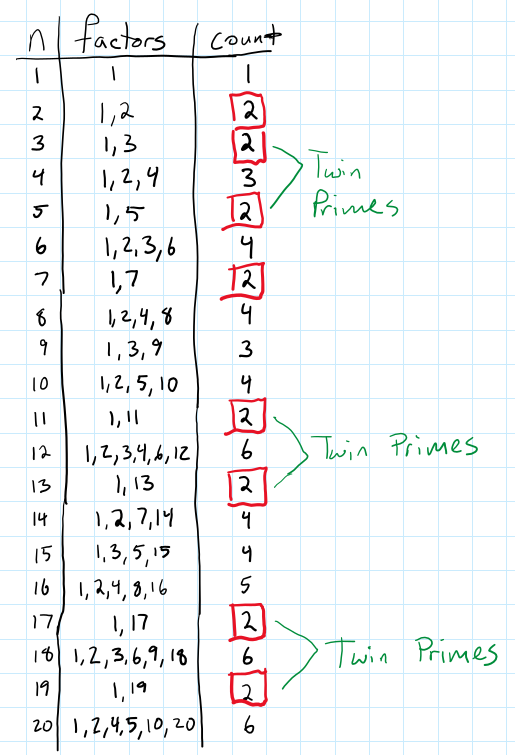
\includegraphics[width=0.3\textwidth]{img/factor-table.png}
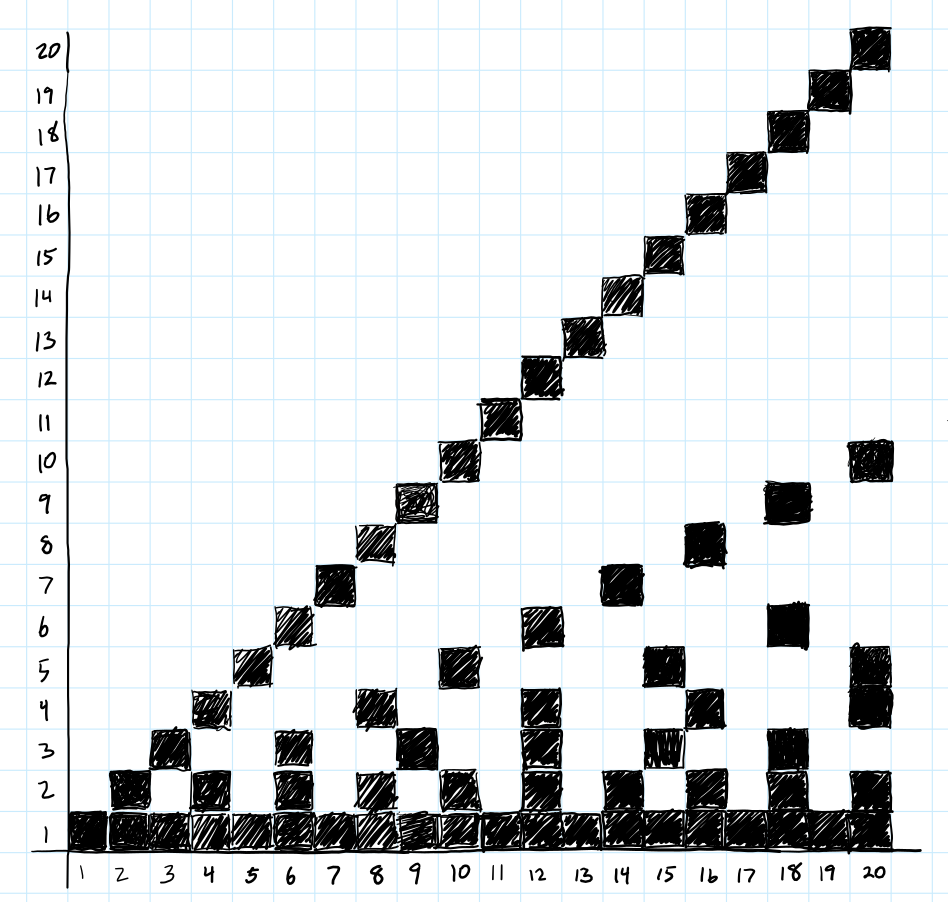
\includegraphics[width=0.5\textwidth]{img/factor-grid.png}





%---------------------------------------------------------------------------
% Bibliography
%---------------------------------------------------------------------------

\addcontentsline{toc}{chapter}{\textcolor{tssteelblue}{Literature}}
\printbibliography{}

%---------------------------------------------------------------------------
% Index
%---------------------------------------------------------------------------

\printindex

\end{document}
